\section{引言}
% 在大数据的时代,人们越来越依赖于数据分析进行决策。例如,当一家超市想要合理进货以便最大化其利润时,他需要考虑超市历史的售卖订单、市场上客户对于商品的喜爱度、各类商品的利润率等方面,这往往需要通过分析各个方面大量的数据来做决定。
在大数据时代,人们越来越依赖数据分析进行决策~\cite{albright2020business}。
% For instance, when a supermarket aims to optimize its profits through informed inventory management, it needs to consider various factors, such as historical sales orders, customer preferences, profit margins for different items. This often necessitates the analysis of a vast amount of data from various aspects to make informed decisions.
% 为了完成数据分析任务,那些没有服务器的人通常把数据分析的任务托管到云服务器上。但在使用云服务器进行数据分析的同时,人们会担心这些重要的数据遭到泄漏,因为这个数据往往涉及到个人的隐私、商业机密等。
为了执行数据分析,没有自己服务器的个人通常将数据分析任务委托给云服务器~\cite{sandhu2021big}。然而,在使用云服务器进行数据分析时,人们担心这些关键数据可能被泄露~\cite{purohit2013data},因为它通常涉及个人隐私或商业机密。
% 为了避免数据的泄漏的问题,越来越多的相关技术被提出以解决数据泄露的问题。这些技术包括:多方安全计算、同态加密、联邦学习、可信执行环境等。
为了解决数据泄露问题,越来越多的相关技术被提出。这些技术包括:安全多方计算(MPC)~\cite{lindell2020secure,patra2021aby2,dalskov2022fast}、同态加密(HE)~\cite{marcolla2022survey,lu2021pegasus,bossuat2021efficient}、联邦学习(FL)~\cite{li2021survey,bonawitz2017practical,shayan2020biscotti}、可信执行环境(TEE)~\cite{zheng2021survey,tsai2017graphene,priebe2018enclavedb}。
% 在这些技术中,MPC和HE具备极高的安全性,因为它是密码学安全的,但由于MPC和HE包含了复杂的密码学操作,其性能相较于其他几类技术表现极差。FL常见于机器学习的场景,主要用于联合建模,对于一般的数据分析场景并不适用。TEE满足各类通用计算的场景,其计算性能较高,但其基于硬件的安全性,相较于MPC和HE的密码学安全,其安全性更低,而且经常出现新发现的基于TEE的侧信道攻击。
在这些技术中,MPC和HE提供极高的安全性,因为它们基于密码学安全原则。然而,由于涉及复杂的密码学操作,与其他类别相比,它们的性能显著较低~\cite{alaya2020homomorphic,evans2018pragmatic}。FL常见于机器学习场景,主要用于协作建模~\cite{li2021survey},可能不太适合典型的数据分析设置。TEE具有通用性,适用于各种通用计算场景,并提供更高的计算性能。然而,其基于硬件的安全性,与MPC和HE的密码学安全性相比较低,并且容易受到新发现的侧信道攻击~\cite{nilsson2020survey}。

% 然而,随着数据分析的场景越来越复杂,现有的这些技术不能直接应用于那些复杂的场景,来解决数据泄漏的问题。
然而,随着涉及多个角色的数据分析场景日益复杂,现有技术无法直接应用于这些复杂场景来有效解决数据泄露问题。
% 现有的数据分析场景中,仅存在租户和云计算服务提供商两个角色,现有技术主要是为了防止云计算服务提供商泄漏租户的数据。但是现在的数据分析场景中,包含了数据提供方、数据使用方、模型提供方、云计算服务提供商这些角色,数据需要防止被数据提供方之外的所有角色泄漏。除此之外,还需要维护数据分析场景中各方的权益,例如,数据使用方得到合理的分析结果,数据提供方、模型提供方、云计算服务提供商获得相应的收益。
% 通过图更形象地描述场景的复杂?
在现有的数据分析场景中,只有两个角色,如图~\ref{fig:analysis_scenarios}(a)所示:租户和云服务提供商。现有技术主要专注于防止云服务提供商泄露租户数据。然而,在当今的数据分析场景中,涉及多个角色,如图~\ref{fig:analysis_scenarios}(b)所示,包括数据提供方、数据使用方、模型提供方和云服务提供商。数据必须防止被数据提供方之外的所有方泄露。除此之外,还需要保护数据分析场景中所有相关方的利益。例如,数据使用方应该获得公平有效的分析结果,而数据提供方、模型提供方和云服务提供商应该进行公平的收入分配。

% 因此,在针对复杂的数据分析场景时,我们需要检测数据使用方是否通过输出的计算结果中包含敏感信息以泄漏数据,模型提供方是否通过恶意的模型泄漏数据,云计算服务提供商通过篡改hypervisor、操作系统、内存、磁盘等泄漏数据,数据提供方、模型提供方以及云计算服务提供商共同生成的计算结果是否合法。
因此,在处理涉及多个角色的数据分析场景时,我们需要检测数据使用方是否试图通过从计算结果中提取敏感信息来泄露数据,模型提供方是否通过恶意模型进行数据泄露,云服务提供商是否通过操纵虚拟机监控程序、操作系统、内存、磁盘等方式进行数据泄露,以及数据提供方、模型提供方和云服务提供商共同生成的计算结果是否合法。

% 很多相关的研究被提出,来解决复杂的数据分析场景时所面临的问题,包括SDTE,PrivacyGuard等。
许多相关研究被提出来解决多角色数据分析场景中面临的挑战,包括SDTE~\cite{dai2019sdte}、PrivacyGuard~\cite{xiao2020privacyguard}、SPDS~\cite{wang2020spds}、Amanuensis~\cite{hardin2022amanuensis}等。
SDTE~\cite{dai2019sdte}在数据交易行业引入了一种称为"数据处理即服务"的创新模型。利用这个模型,它通过一系列交易协议实现安全的数据交易。
PrivacyGuard~\cite{xiao2020privacyguard}利用智能合约定义数据使用策略,并利用TEE进行高效的合约执行,同时保护私有数据。
SPDS~\cite{wang2020spds}与PrivacyGuard类似,使用智能合约定义数据使用策略,并实现两阶段交付协议以确保计算结果和支付的安全发布。
Amanuensis~\cite{hardin2022amanuensis}探索了区块链技术和TEE的交集,以解决数据共享中的数据溯源、机密性和用户隐私挑战。

\begin{figure}[t]
  \centering
{
\begin{tabular}{cc}
      \subfloat[租户和云服务提供商]{
  \hspace*{-0.7cm}
        \scalebox{0.42}{
        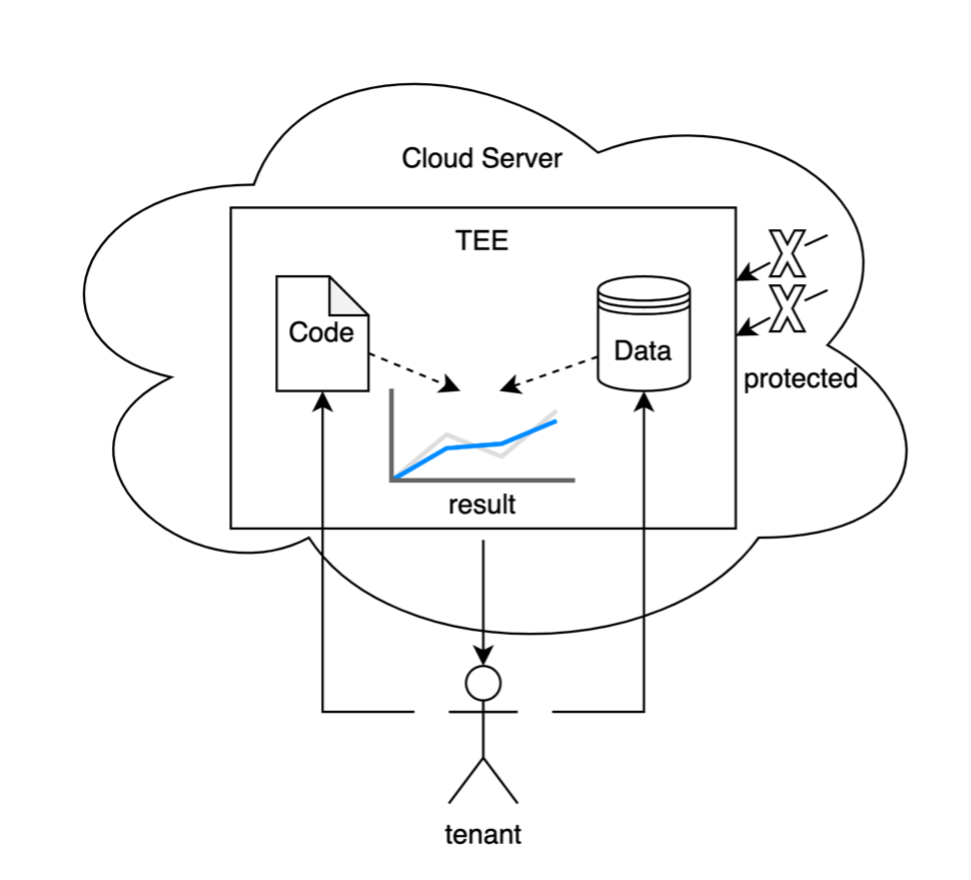
\includegraphics{images/analysis_2_roles.png}
        }
      } &
      \subfloat[多角色]{
  \hspace*{-1cm}
        \scalebox{0.42}{
        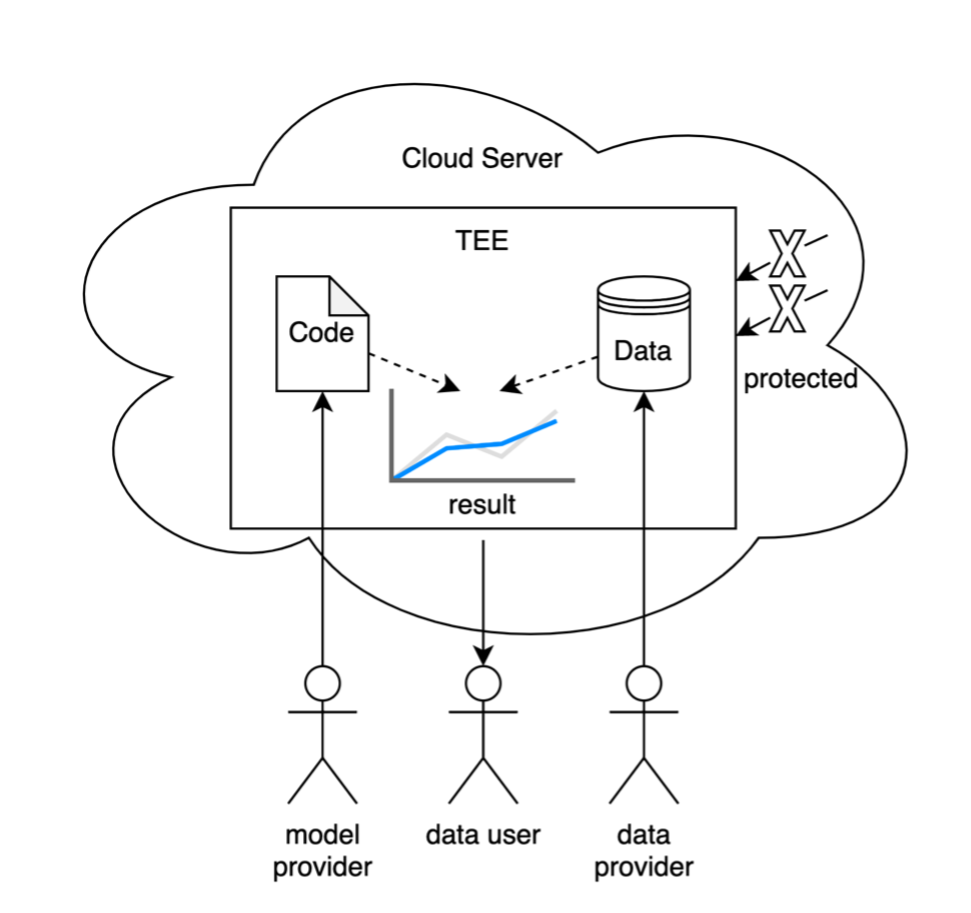
\includegraphics{images/analysis_4_roles.png}
        }
      }    \\
\end{tabular}
  }
  \caption{\small 两个角色与多角色的数据分析场景。}
  \label{fig:analysis_scenarios}
\end{figure}
% 然而,这些相关的研究在解决复杂的数据分析场景时,仍存在一些限制。
然而,这些相关研究在解决这些数据分析场景时仍存在某些限制。
% 首先,这些相关的研究工作不能保证数据分析结果中不会泄漏数据。虽然这些工作引入了数据使用规则,用以描述哪些人以什么样的价格访问哪些类型的数据,但对数据进行分析的程序是存在作恶的可能的,分析程序的最终输出结果可能是包含敏感信息泄漏的。一个最简单的例子是,分析程序直接输出原始数据,这样数据分析结果就获取到了完整的原始数据。
首先,这些相关研究工作不能保证数据分析结果中不会泄露数据。虽然这些工作引入了数据使用策略来描述谁可以以什么价格访问什么类型的数据,但数据分析程序存在恶意行为的可能性。分析程序的最终输出可能包含敏感信息的泄露。一个例子是当分析程序直接输出原始数据时,允许数据分析结果获得完整的原始数据。
% 一个straghtforward的解决方案是,要求分析程序公开,数据提供方可以审核分析程序是否存在泄漏数据的代码。但是对于模型提供方而言,模型也是他们重要的资产,他们不希望模型公开。另一方面,对于复杂的分析程序来说,审核分析程序存在巨大的工作量,不可能要求每一个分析任务都去进行审核,这会大大降低数据分析的效率。
一个直接的解决方案是要求分析程序公开,供数据提供方审计,确保它不包含可能导致数据泄露的代码。然而,对于模型提供方来说,他们的模型是有价值的资产,他们可能不愿意公开。另一方面,审计复杂的分析程序代表巨大的工作量,要求对每个分析任务进行审计是不可行的,因为这会显著降低数据分析的效率。

% 结果可验证
% 其次,当前的工作中并不能保证计算结果的可信与可验证。具体来说,数据使用方得到计算结果后,他不能确定这个计算结果确实是通过指定的数据与指定的模型运行之后得到的计算结果,而不是一个随机生成的结果。更进一步,数据使用方并没有任何方式去验证这个结果的正确性。如果计算结果的可信和可验证都无法保证,那么完全可以用一个伪造的计算结果来欺骗数据使用方,数据使用方的利益将会受到损害。
其次,现有工作无法确保计算结果的可靠性和可验证性。具体来说,当数据使用方收到计算结果时,他们无法确认这些结果确实来自通过指定模型运行指定数据,而不是简单随机生成的。此外,数据使用方缺乏任何验证这些结果正确性的方法。如果没有对计算结果的可靠性和可验证性的保证,就有可能使用欺骗性结果来误导数据使用方,损害他们的利益。

% 分析程序一致性
% 最后,当前的工作中每一次进行数据分析任务都需要使用remote attestation来保证分析程序的一致性,但是有相关工作表明,remote attestation具有低效、依赖可信第三方的缺点。
最后,在现有工作中,每个数据分析任务都需要使用远程认证来确保分析程序的一致性。然而,相关工作~\cite{chen2019opera,chen2022mage}表明,远程认证具有低效和依赖可信第三方的缺点。
% 以Intel SGX中的Enhanced Privacy ID(EPID)为例,一次remote attestation的过程会涉及到Intel Provisioning Service(IPS)、Intel Attestation(IAS) Service、Intel-signed provisioning enclave(PvE)、Intel-signed quoting enclave(QE)以及分析程序Enclave之间的交互。这些服务和Enclaves之间的交互需要通过广域网传输数据,同时,传输的数据需要加密保证其安全性,对于频繁的数据分析任务而言,性能上会有较大的损失。另一方面,IPS和IAS是Intel提供的中心化服务,remote attestation需要依赖其稳定运行。
以Intel软件保护扩展(SGX)增强隐私ID(EPID)为例,单次远程认证过程涉及Intel配置服务(IPS)、Intel认证服务(IAS)、Intel签名的配置enclave(PvE)、Intel签名的引用enclave(QE)和分析程序enclave之间的交互。这些交互需要通过广域网传输数据,传输的数据必须加密以确保其安全性。对于频繁的数据分析任务,这可能导致显著的性能开销。另一方面,IPS和IAS是Intel提供的集中式服务,使远程认证依赖于它们的稳定运行。

在本文中,我们提出了Fidelius,一个利用Intel SGX和区块链来增强数据分析安全性的系统,解决了前面提到的局限性。
% 其中,Intel SGX保证数据分析过程的security和integrity,区块链用于可信的传输、存储和验证。
Intel SGX确保数据分析过程的安全性和完整性,而区块链用于可信的传输、存储和验证。

% 为了解决计算结果泄漏数据的问题,Fidelius使用了静态二进制分析的方法,检查模型提供方的分析程序是否遵循隐私描述语言。其中,我们引入的隐私描述语言将数据的运算规则描述为有限状态机,反映了从输入数据到输出数据的状态转换,不在隐私描述语言描述的状态转换,都会被认为违反了隐私规则。
为了解决计算结果中数据泄露的问题,Fidelius采用静态二进制分析方法~\cite{schulte2019gtirb}来检查模型提供的分析程序是否遵循隐私描述语言(PDL)。在这种情况下,引入的PDL将数据的计算规则描述为有限状态机(FSM),捕获从输入数据到输出数据的状态转换。任何未在PDL中描述的状态转换都被视为违反隐私规则。

% 为了解决计算结果的可信与可验证的问题,Fidelius提供了一套密码协议,该协议中由数据使用方提供一个私钥,该私钥通过加密转发至分析程序的Enclave中,并签名计算结果。由于该私钥仅在指定的分析程序Enclave中解密获得,数据提供方、模型提供方、云计算服务提供商均无法获取,故只要被签名的计算结果能够通过验证,说明计算结果确实出自指定的分析程序且可验证。
为了确保计算结果的可靠性和可验证性,Fidelius提供了一个密码协议。在这个协议中,数据使用方提供一个私钥,该私钥安全地传输到分析程序的Enclave中并用于签名计算结果。由于这个私钥只能在指定的分析程序Enclave内解密,数据提供方、模型提供方和云服务提供商都无法访问。因此,如果签名的计算结果能够成功验证,就确认结果确实来自指定的分析程序并且是可验证的。

% 为了解决remote attestation低效、持续依赖中心化服务的问题,Fidelius结合设计的密码协议以及local attestation实现分析程序的一致性验证。Fidelius设计了密钥管理的Enclave,在初始化的过程中获取密钥的授权,在此后的所有数据分析任务中,使用该经授权的密钥执行local attestation完成分析程序的一致性验证。
为了解决远程认证的低效和持续依赖集中式服务的问题,Fidelius结合设计的密码协议和本地认证来实现分析程序的一致性验证。Fidelius引入了密钥管理Enclave,在初始化过程中获得授权密钥。随后,在所有数据分析任务中,使用这个授权密钥执行本地认证,确保分析程序的一致性。

本文的主要贡献总结如下:
\begin{itemize}
    \item 首先,我们引入隐私描述语言(PDL)结合静态二进制分析,严格强制执行数据机密性,防止计算结果中的敏感数据泄露。
    \item 其次,我们设计了一种密码协议来确保计算结果的可靠性和可验证性。
    \item 我们集成了密码协议与本地认证机制,确保在受保护环境中执行的分析程序的完整性和正确性。
    \item 最后,我们评估了Fidelius的性能,实验结果表明它产生的开销最小,对数据分析系统的贡献不到2\%,同时超越现有解决方案30倍以上。
\end{itemize} 